\chapter{Backward compatibility} \label{Chp:Backward}

The development environment of \dfastmi includes an automated test bench for regression testing.
Many of the tests executed are unit tests to validate the functionality of individual routines/objects.
See \citet{trm} for details.
The regression test bed also includes a number of system/acceptance tests executing the complete \dfmi analysis.
Those tests comprise both the new \emph{stepped-hydrograph} approach as well as the traditional 3 discharges approach of WAQMORF.
The latter is available in \dfmi 3 as backward compatibility mode.

For testing that backward compatibility mode the following cases are currently used:

\begin{itemize}
\item \nameref{Sec:GendtseWaard_backward}
%\item Rijntakken II
%\item Rijntakken III (optioneel)
\item \nameref{Sec:DeLymen_backward}
\end{itemize}

\begin{Remark}
\item There are slight differences in spaces/empty lines between WAQMORF and \dfmi.
\item All zero-values are reported as \keyw{0.000} by WAQMORF, but \dfmi reports \keyw{0.000} or \keyw{-0.000} depending on the sign of the actual (non-rounded) value.
\item All results of \dfmi when running in \keyw{cli} mode are equal to those of WAQMORF.
When \dfmi running in batch mode using the configuration settings of \dfmi version 2 (configuration files marked as version 1.0), the report and year-averaged bed level changes are also equal to those of WAQMORF.
However, the minimum and maximum bed level change are defined differently.
WAQMORF (and the backward compatible \dfmi{} \keyw{cli} mode) define them as the bed level change after the low flow and high flow period respectively.
\dfmi{} \keyw{batch} and \keyw{gui} modes define them as the point-wise minimum and maximum of bed level changes throughout the year.
\end{Remark}

\section{Gendtse Waard}\label{Sec:GendtseWaard_backward}

\emph{The input files of this case are included in the distribution under \file{examples\_compatibility/01 - Gendtse Waard}.}

This concerns a secondary channel located at the "Gendtse Waard" along the Bovenwaal, a stretch of the river Waal.
This case is based on Delft3D simulations carried out by \citet{Ottevangeretal2016}.
All tests have been completed successfully.
The results obtained using \dfmi 3 are equal to those obtained using WAQMORF when WAQUA data files are used as input.
The results obtained using \dfmi 3 are identical to those obtained using \dfmi 2 when UGRID netCDF files are used as input. 
The results obtained using UGRID netCDF files are identical to those obtained using WAQUA data files (ignoring the change in data formats used).
The computed morphological impact is shown in \autoref{fig:backward1.png}.

\begin{figure}[H]
\center
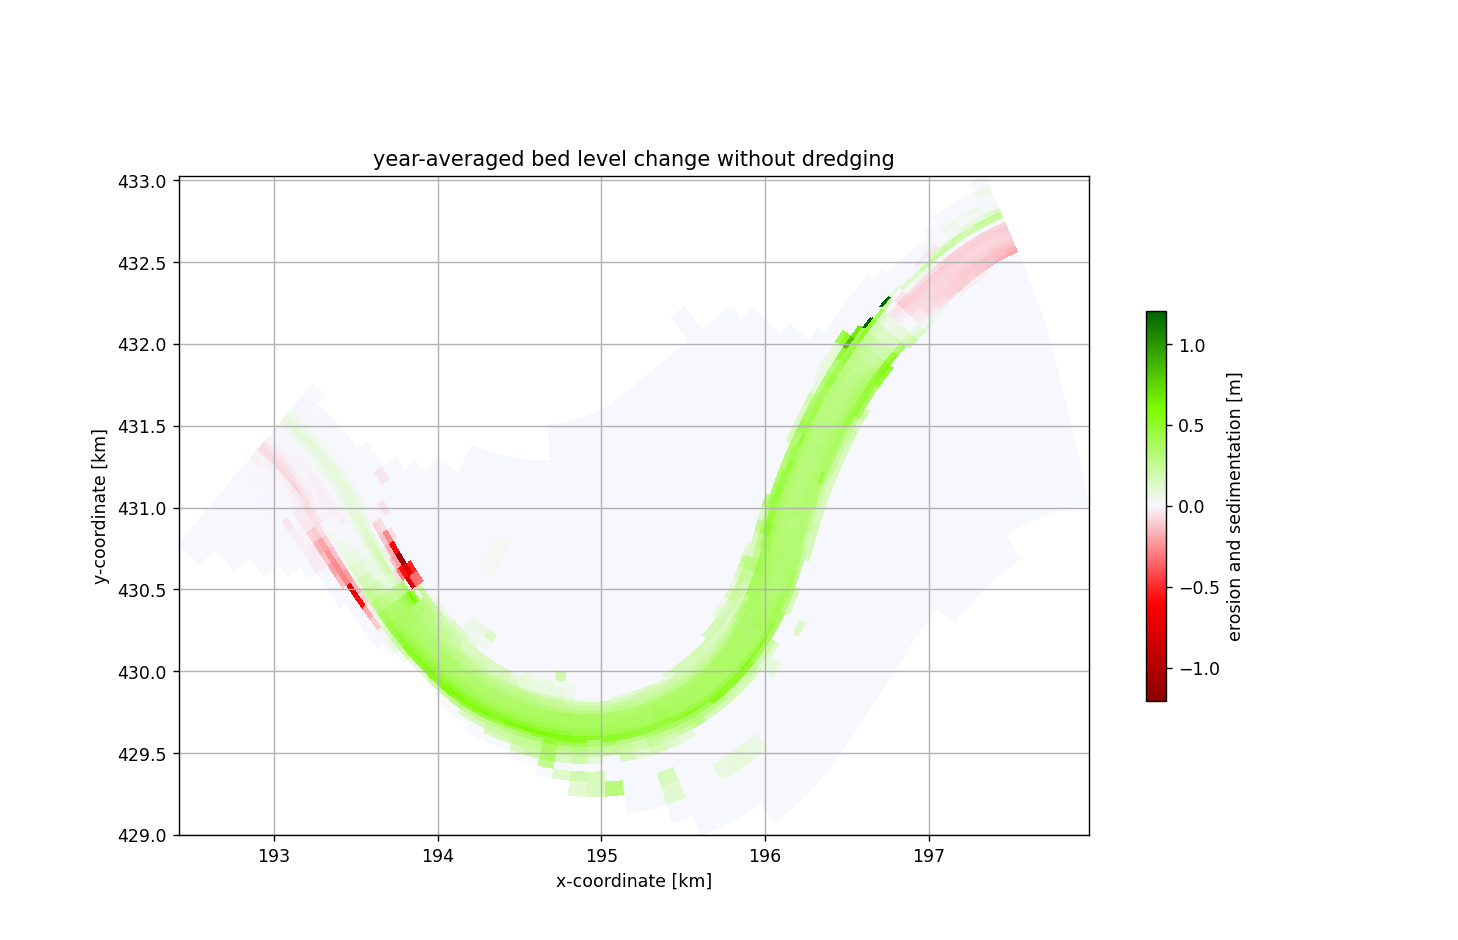
\includegraphics[width=12cm]{figures/report_Figure1.png}
\caption{Morphological impact of the side channel "Gendtse Waard".
Default figure generated by \dfmi.}
\label{fig:backward1.png}
\end{figure}

\section{De Lymen}\label{Sec:DeLymen_backward}

\emph{The input files of this case are included in the distribution under \file{examples\_compatibility/02 - De Lymen}.}

This concerns a section of the "Bedijkte Maas" between Batenburg and Appeltern, along the river Meuse.
An impression of the intervention is given in \autoref{fig:backward2.png}.
For this case only the pure regression test against WAQMORF results has been performed.
The results obtained using \dfmi 3 are equal to those obtained using WAQMORF when WAQUA data files are used as input.

\begin{figure}[H]
\center
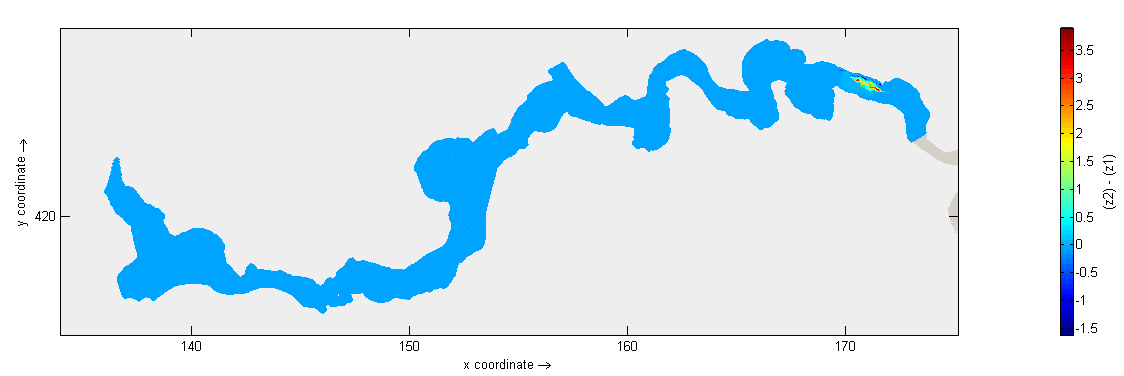
\includegraphics[width=12cm]{figures/Lymen_dz.png}
\caption{Change in floodplain elevation for "De Lymen".
Visualized using QUICKPLOT.}
\label{fig:backward2.png}
\end{figure}